%%%%%%%%%%%%%%%%%%%%%%%%%%%%%%%%%%%%%%%%%%%%%%%%%%%%%%%%%%%%%%%%
%%                                                            %%
%% latinProseComposition, Italian translation 2016.12 - 2017  %%
%%                                                            %%
%% From:  Henry Carr Pearson, Latin Prose Composition         %%
%%        (1903, New York, American Book Company)             %%
%%                                                            %%
%%    https://archive.org/details/latinprosecompo01peargoog   %%
%%                                                            %%
%% Translated by g.p.ciceri <gp.ciceri@gmail.com>             %%
%% ---------------------------------------------------------- %%
%% This translation is Licensed under                         %%
%% Creative Commons Attribution-ShareAlike 4.0 International  %%
%% https://creativecommons.org/licenses/by-sa/4.0/            %%
%%                                                            %%
%%%%%%%%%%%%%%%%%%%%%%%%%%%%%%%%%%%%%%%%%%%%%%%%%%%%%%%%%%%%%%%%

% āēīōū
% ăĕĭŏŭ




\documentclass[nols]{tufte-handout}

%\geometry{showframe} % display margins for debugging page layout

\usepackage{fontspec}
\usepackage{ifxetex}
\setmainfont[Path=./fonts/palatino-linotype/, ItalicFont=palai.ttf, BoldFont=palab.ttf]{pala.ttf}


% \defaultfontfeatures{Mapping=tex-text}
% \setromanfont[Path=./fonts/TeX-Gyre-Schola/,Mapping=tex-text]{TeX Gyre Schola}
% \setsansfont[Path=./fonts/TeX-Gyre-Heros/,Scale=MatchLowercase,Mapping=tex-text]{TeX Gyre Heros}
% \setmonofont[Path=./fonts/TeX-Gyre-Cursor/,Scale=MatchLowercase]{TeX Gyre Cursor}

\usepackage{lipsum}
\usepackage{url}
\usepackage{longtable}
\usepackage{stackengine}

\usepackage{graphicx} % allow embedded images
  \setkeys{Gin}{width=\linewidth,totalheight=\textheight,keepaspectratio}
  \graphicspath{{graphics/}} % set of paths to search for images
\usepackage{amsmath}  % extended mathematics
\usepackage{booktabs} % book-quality tables
\usepackage{units}    % non-stacked fractions and better unit spacing
\usepackage{multicol} % multiple column layout facilities
\usepackage{lipsum}   % filler text
\usepackage{fancyvrb} % extended verbatim environments
  \fvset{fontsize=\normalsize}% default font size for fancy-verbatim environments

% Standardize command font styles and environments
\newcommand{\doccmd}[1]{\texttt{\textbackslash#1}}% command name -- adds backslash automatically
\newcommand{\docopt}[1]{\ensuremath{\langle}\textrm{\textit{#1}}\ensuremath{\rangle}}% optional command argument
\newcommand{\docarg}[1]{\textrm{\textit{#1}}}% (required) command argument
\newcommand{\docenv}[1]{\textsf{#1}}% environment name
\newcommand{\docpkg}[1]{\texttt{#1}}% package name
\newcommand{\doccls}[1]{\texttt{#1}}% document class name
\newcommand{\docclsopt}[1]{\texttt{#1}}% document class option name
\newenvironment{docspec}{\begin{quote}\noindent}{\end{quote}}% command specification environment

% concetti morfosintattici
\usepackage{xspace} 
\newcommand{\noun}{\textsc{sostantivo}\xspace}
\newcommand{\nouns}{\textsc{sostantivi}\xspace}
\newcommand{\adject}{\textsc{aggettivo}\xspace}
\newcommand{\adjects}{\textsc{aggettivi}\xspace}
\newcommand{\gnumber}{\textsc{numero}\xspace}
\newcommand{\gnumbers}{\textsc{numeri}\xspace}
\newcommand{\gender}{\textsc{genere}\xspace}
\newcommand{\genders}{\textsc{generi}\xspace}
\newcommand{\gcase}{\textsc{caso}\xspace}
\newcommand{\gcases}{\textsc{casi}\xspace}
\newcommand{\tense}{\textsc{tempo}\xspace}
\newcommand{\mood}{\textsc{modo}\xspace}
\newcommand{\gverb}{\textsc{verbo}\xspace}
\newcommand{\gverbs}{\textsc{verbi}\xspace}
\newcommand{\adjective}{\textsc{aggettivo}\xspace}
\newcommand{\nom}{\textsc{nom}\xspace}
\newcommand{\gen}{\textsc{gen}\xspace}
\newcommand{\dat}{\textsc{dat}\xspace}
\newcommand{\acc}{\textsc{acc}\xspace}
\newcommand{\voc}{\textsc{voc}\xspace}
\newcommand{\abl}{\textsc{abl}\xspace}
\newcommand{\gexit}{\textsc{uscita}\xspace}
\newcommand{\gexits}{\textsc{uscite}\xspace}
\newcommand{\declinazione}{\textsc{declinazione}\xspace}
\newcommand{\masc}{\textsc{maschile}\xspace}
\newcommand{\femm}{\textsc{femminile}\xspace}
\newcommand{\neut}{\textsc{neutro}\xspace}

\newcommand{\indic}{\textsc{indicativo}\xspace}
\newcommand{\imper}{\textsc{imperativo}\xspace}
\newcommand{\gcong}{\textsc{congiuntivo}\xspace}
\newcommand{\ott}{\textsc{ottativo}\xspace}
\newcommand{\partic}{\textsc{participio}\xspace}
\newcommand{\infin}{\textsc{infinito}\xspace}

\newcommand{\pres}{\textsc{presente}\xspace}
\newcommand{\imperf}{\textsc{imperfetto}\xspace}
\newcommand{\aor}{\textsc{aoristo}\xspace}
\newcommand{\fut}{\textsc{futuro}\xspace}
\newcommand{\perf}{\textsc{perfetto}\xspace}
\newcommand{\pperf}{\textsc{piuccheperfetto}\xspace}

\newcommand{\sing}{\textsc{singolare}\xspace}
\newcommand{\plur}{\textsc{plurale}\xspace}
\newcommand{\dual}{\textsc{duale}\xspace}

\newcommand{\si}{\textsc{sing}\xspace}
\newcommand{\pl}{\textsc{plur}\xspace}
\newcommand{\du}{\textsc{dual}\xspace}

\newcommand{\att}{\textsc{attivo}\xspace}
\newcommand{\med}{\textsc{medio}\xspace}
\newcommand{\pass}{\textsc{passivo}\xspace}
\newcommand{\medpass}{\textsc{medio-passivo}\xspace}


% italianitudini
\renewcommand{\figurename}{Figura}
\renewcommand{\tablename}{Tabella}
\renewcommand{\contentsname}{Indice}

% fix per un qualche problema
\ifxetex
  \newcommand{\textls}[2][5]{%
    \begingroup\addfontfeatures{LetterSpace=#1}#2\endgroup
  }
  \renewcommand{\allcapsspacing}[1]{\textls[15]{#1}}
  \renewcommand{\smallcapsspacing}[1]{\textls[10]{#1}}
  \renewcommand{\allcaps}[1]{\textls[15]{\MakeTextUppercase{#1}}}
  \renewcommand{\smallcaps}[1]{\smallcapsspacing{\scshape\MakeTextLowercase{#1}}}
  \renewcommand{\textsc}[1]{\smallcapsspacing{\textsmallcaps{#1}}}
\fi

% too many float...
\extrafloats{100}

\title{Latin Prose Composition. Per scrivere in Latino. \newline Lezione II - Il caso Accusativo).}

\author[gpciceri]{a cura di Milagathòs: Milo's help to enjoy humanities\marginnote{\url{http://www.milagathos.com}}
}

\date{18 Gennajo 2017} % without \date command, current date is supplied


\begin{document}

\maketitle% this prints the handout title, author, and date

\begin{marginfigure}[-2.5cm]
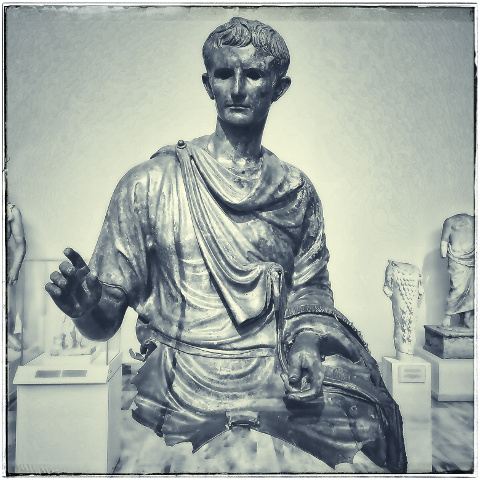
\includegraphics{smallthumb-lesson_I.jpeg}
\setfloatalignment{b}
\end{marginfigure}


\begin{abstract}
\noindent
Queste lezioni riprendono la prima parte del manuale di composizione latina di Pearson\cite{pearson1903}, del quale seguono la numerazione;
la struttura della lezione è piuttosto regolare: ad un sintetico \textsc{richiamo morfosintattico} fanno seguito delle \textsc{frasi di esempio},
vi sono poi \textsc{riferimenti al testo di grammatica} (qui sono riportati solo quelli al testo di Harkness\cite{harkness1898}, con relativa numerazione [H nnn.]) 
dove le regole grammaticali sono spiegate per esteso e, alla fine della lezione, 
un \textsc{esercizio di composizione in latino} - delle brevi frasi da tradurre.

\bigskip
\noindent
Lezione II: utilizzi del caso Accusativo; esempi, esercizi.
\end{abstract}

%\printclassoptions

\newthought{12.} L'oggetto diretto di un verbo transitivo viene espresso con il caso \textsc{Accusativo}: 
\\
\vspace{0.5em}
\hangindent=2em \textbf{librum scripsit,} \textit{scrisse un libro}. 

\newthought{13. Accusativo Cognato.} Il significato di un verbo, anche di norma intransitivo, può essere enfatizzato o meglio definito aggiungendo un oggetto di derivazione correlata. Questo costrutto è detto \textit{Accusativo Cognato} e l'oggetto è di solito precisato da un aggettivo:
\\
\vspace{0.5em}
\hangindent=2em \textbf{tutam vitam vivere,} \textit{condurre una vita sicura}.

\newthought{14. Accusativo Predicativo.} Molti verbi che indicano azioni di \textit{fare, scegliere, nominare, mostrare, ecc.} possono reggere due accusativi - uno della persona o cosa oggetto del verbo, l'altro come predicato del verbo stesso:
\\
\vspace{0.5em}
\hangindent=2em \textbf{urbem Romam vocavit,} \textit{chiamò la città Roma}.
 
\newthought{15. Doppio Accusativo.} Alcuni verbi che indicano azioni di \textit{chiedere, domandare, insegnare, nascondere, ecc.} possono reggere due accusativi - uno per la persona, l'altro per la cosa:
\\
\vspace{0.5em}
\hangindent=2em \textbf{pacem te poscimus,} \textit{chiediamo pace a te}.

\newthought{Osservazioni}
\begin{itemize}
\item[\textsc{1.}] Alcuni di questi verbi possono reggere l'ablativo della persona con una preposizione, al posto dell'accusativo. Così, in genere, \textbf{peto (ab),} \textit{cercare (da)}; \textbf{postulo (ab),} \textit{domandare (di)}; \textbf{quaero (ab, de, ex),} \textit{chiedere (di)}:
\\
\vspace{0.5em}
\hangindent=2em \textbf{quaerit ex solo ea,} \textit{gli chiede in privato a proposito di queste cose}.\\
\hangindent=2em \textbf{pacem a vobis petimus,} \textit{cerchiamo pace da voi}.
\end{itemize}

\newthought{16. Accusativo di Tempo e Spazio.} L'accusativo è usato per esprimere \textit{la durata di un tempo} e \textit{l'estensione di uno spazio}:
\\
\vspace{0.5em}
\hangindent=2em \textbf{fossas quindecim pedes latas,} \textit{fossati ampi quindici passi}.\\
\hangindent=2em \textbf{quadraginta annos vixit,} \textit{visse (per) quarant'anni}.

\newthought{Osservazioni}
\begin{itemize}
\item[\textsc{1.}] Qualche volta viene aggiunta, per enfasi, la preposizione \textbf{per}, come in:
\\
\vspace{0.5em}
\hangindent=2em \textbf{ludi per decem dies,} \textit{giochi per dieci giorni}.
\end{itemize}

\newthought{17. Accusativo di Moto a Luogo.} Nomi propri di città, di piccola isola o di piccola penisola sono messi all'\acc per indicare \textit{la destinazione} o \textit{il limite} verso il quale è diretto il moto espresso dal verbo:
\\
\vspace{0.5em}
\hangindent=2em \textbf{missi legati Athenas sunt,} \textit{gli ambasciatori furono mandati ad Atene}.\\
\hangindent=2em \textbf{quadraginta annos vixit,} \textit{visse (per) quarant'anni}.

\newthought{Osservazioni}
\begin{itemize}
\item[\textsc{1.}] Con lo lo stesso significato vengono usati gli \acc \textbf{domum} e \textbf{rus}:
\\
\vspace{0.5em}
\hangindent=2em \textbf{domum reductus est,} \textit{fu condotto a casa}.\\
\hangindent=2em \textbf{ego rus ibo,} \textit{andrò in (quel) paese}.
\item[\textsc{2.}] Con tutte le altre denominazioni di luoghi si richiede una preposizione \textbf{ad, in} per indicare la destinazione del moto:
\\
\vspace{0.5em}
\noindent \hangindent=2em \textbf{in Italiam venit,} \textit{arrivò in Italia}.\\
\noindent \hangindent=2em \textbf{legiones ad urbem adducit,} \textit{conduce le legioni verso la città}.
\item[\textsc{3.}] Quando \textbf{domum} è precisato in un qualsiasi modo, eccetto tramite un pronome o un genitivo possessivo, si usa di norma la preposizione \textbf{in}:
\\
\vspace{0.5em}
\hangindent=2em \textbf{in illam domum,} \textit{(entrò) in quella casa}.\\
\hangindent=2em \textbf{domos suas,} \textit{(entrarono) nelle loro case}.
\end{itemize}


\newthought{18. Accusativo di Esclamazione.} Un'esclamazione, se precisata da un aggettivo o da un genitivo, può essere espressa in accusativo:
\\
\vspace{0.5em}
\hangindent=2em \textbf{me miserum,} \textit{ah, povero me!}\\
\hangindent=2em \textbf{o fallacem spem,} \textit{oh, speranza mal riposta!}.


\newthought{Riferimenti per l'Accusativo.} vedi [H 403-421.]

\newthought{19. Tradurre in Latino:}
\textsc{1.}~Cesare chiese a loro del grano. \quad
\textsc{2.}~Sceglieranno lui come console. \quad
\textsc{3.}~Povero me, vado a Roma!. \quad
\textsc{4.}~Chiederanno cinquanta navi a loro. \quad
\textsc{5.}~Rimase in città per dieci giorni. \quad
\textsc{6.}~Costruirono un muro alto quindici piedi. \quad
\textsc{7.}~Partì verso casa sua. \quad
\textsc{8.}~Per molti giorni nascose l'impresa a suo padre. \quad
\textsc{9.}~Il nemico marciò in Italia. \quad
\textsc{10.}~Il ragazzo e sua madre furono (resi) liberi.


\begin{figure}[!b]
  %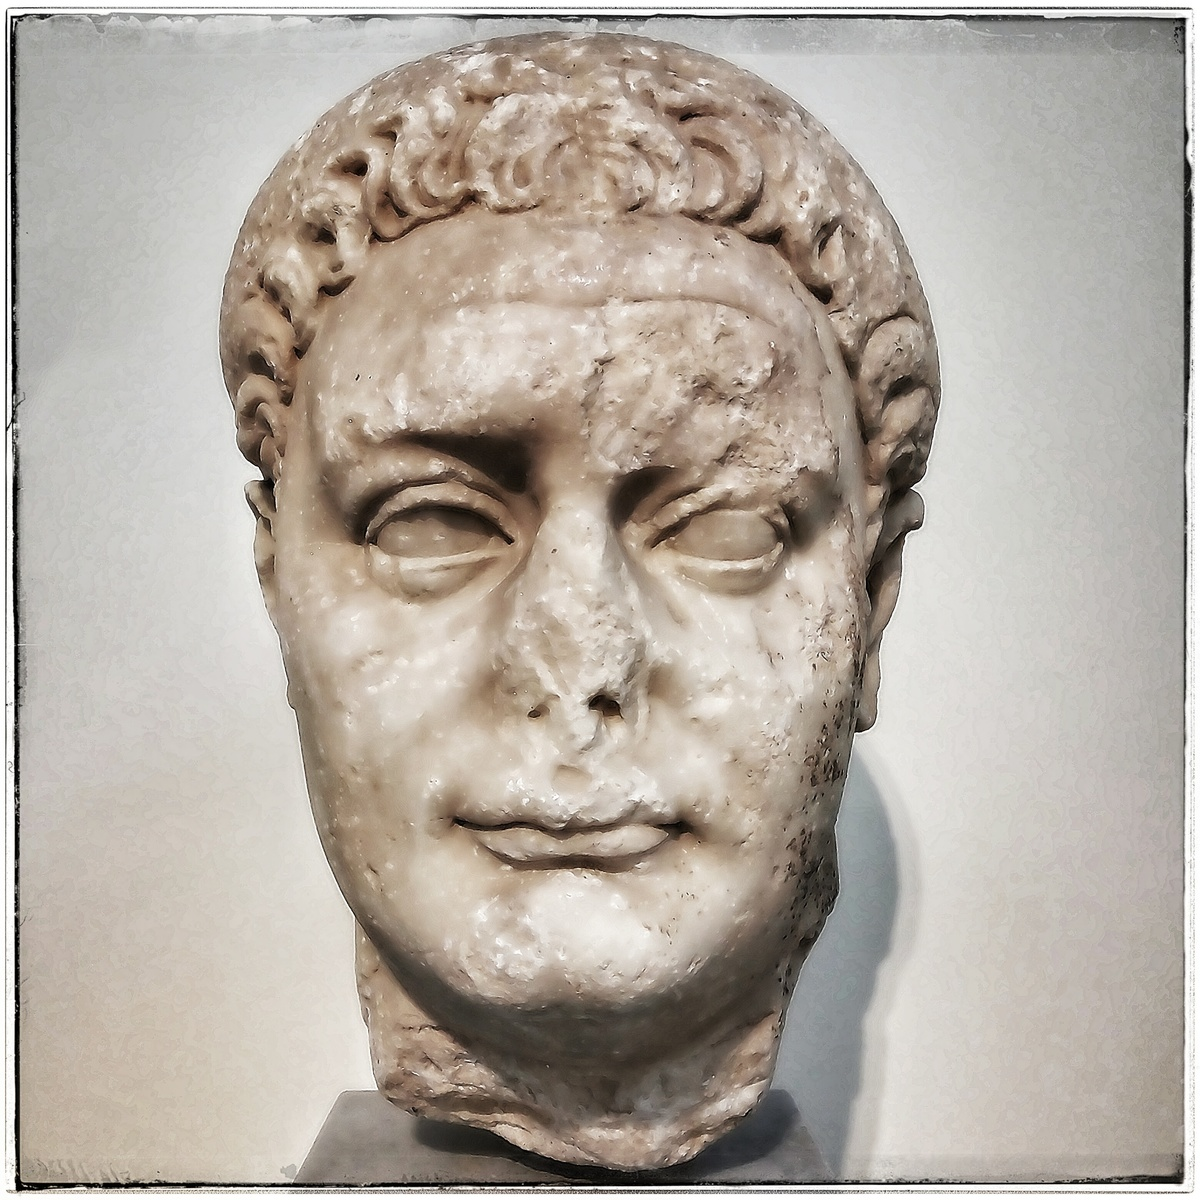
\includegraphics{thumb-lesson_II.jpeg}
  %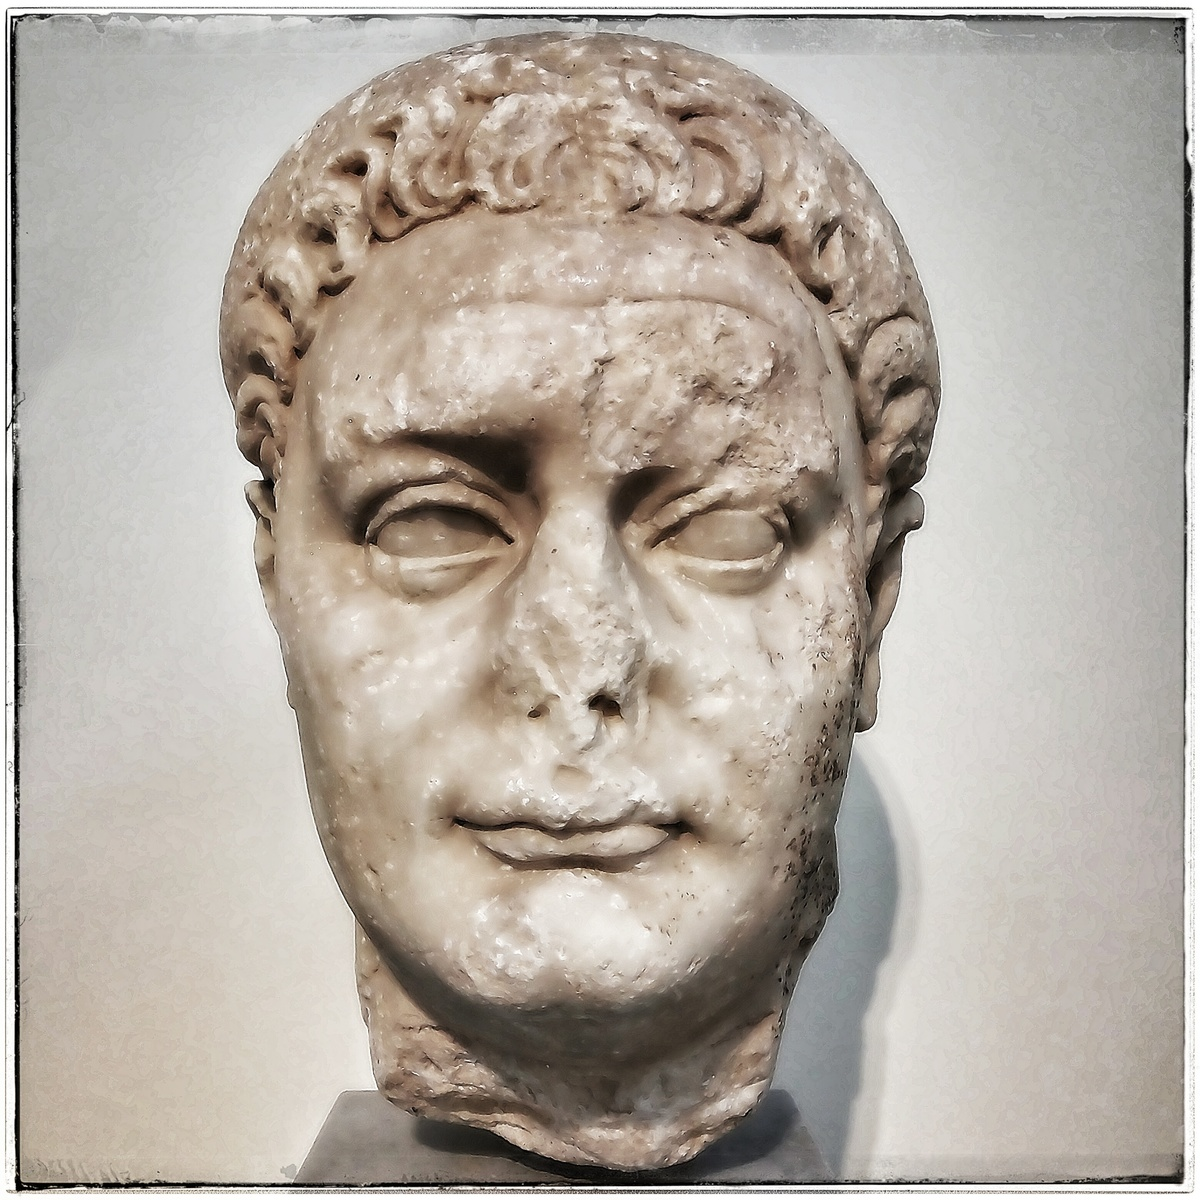
\includegraphics[width=0.9\linewidth]{thumb-lesson_II.jpeg}
  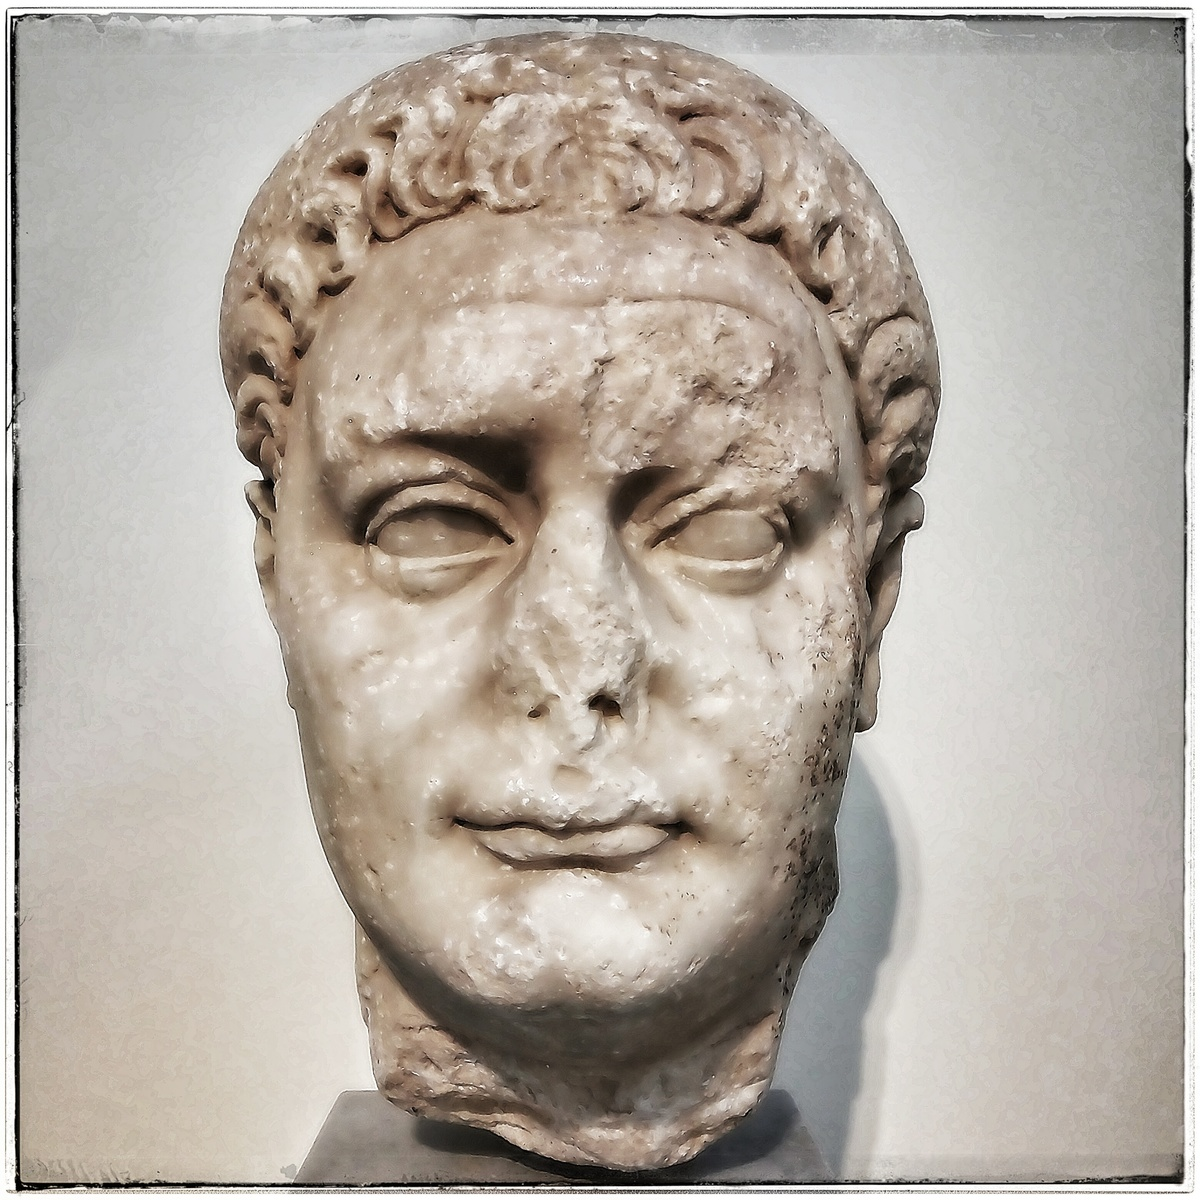
\includegraphics{thumb-lesson_II.jpeg}
  \caption{Museo Nazionale di Archeologia di Atene}
  \label{fig:textfig}
  %\zsavepos{pos:textfig}
  %\setfloatalignment{b}
\end{figure}

 

\nobibliography{latinBiblio}
\bibliographystyle{alpha}


\end{document}
